% -----------------------------------------------
% Template for SMC 2022
% based on SMC 2022 template
% -----------------------------------------------

\documentclass{article}
\usepackage{smc}
\usepackage{times}
\usepackage{ifpdf}
\usepackage[english]{babel}
\usepackage{cite}
%%%% Added by LR
\usepackage{booktabs}
\usepackage{makecell}
\usepackage[utf8]{inputenc} % « guillemets »
\usepackage{tablefootnote}

%%%%%%%%%%%%%%%%%%%%%%%% Some useful packages %%%%%%%%%%%%%%%%%%%%%%%%%%%%%%%
%%%%%%%%%%%%%%%%%%%%%%%% See related documentation %%%%%%%%%%%%%%%%%%%%%%%%%%
%\usepackage{amsmath} % popular packages from Am. Math. Soc. Please use the 
%\usepackage{amssymb} % related math environments (split, subequation, cases,
%\usepackage{amsfonts}% multline, etc.)
%\usepackage{bm}      % Bold Math package, defines the command \bf{}
%\usepackage{paralist}% extended list environments
%%subfig.sty is the modern replacement for subfigure.sty. However, subfig.sty 
%%requires and automatically loads caption.sty which overrides class handling 
%%of captions. To prevent this problem, preload caption.sty with caption=false 
%\usepackage[caption=false]{caption}
%\usepackage[font=footnotesize]{subfig}


%user defined variables
%\def\papertitle{GIHME : Muti-purpose dataset of Guitar Improvisations with Hexaphonic Muti-Effects}
\def\papertitle{Guitar Improvisations with Hexaphonic MultiEffect (GIHME) dataset and practice analysis}
\def\firstauthor{Loïc Reboursière}
\def\secondauthor{Thierry Dutoit}
\def\thirdauthor{Vincent Tiffon}

% adds the automatic
% Saves a lot of output space in PDF... after conversion with the distiller
% Delete if you cannot get PS fonts working on your system.

% pdf-tex settings: detect automatically if run by latex or pdflatex
\newif\ifpdf
\ifx\pdfoutput\relax
\else
   \ifcase\pdfoutput
      \pdffalse
   \else
      \pdftrue
\fi

\ifpdf % compiling with pdflatex
  \usepackage[pdftex,
    pdftitle={\papertitle},
    pdfauthor={\firstauthor, \secondauthor, \thirdauthor},
    bookmarksnumbered, % use section numbers with bookmarks
    pdfstartview=XYZ % start with zoom=100% instead of full screen; 
                     % especially useful if working with a big screen :-)
   ]{hyperref}
  %\pdfcompresslevel=9

  \usepackage[pdftex]{graphicx}
  % declare the path(s) where your graphic files are and their extensions so 
  %you won't have to specify these with every instance of \includegraphics
  \graphicspath{{./figures/}}
  \DeclareGraphicsExtensions{.pdf,.jpeg,.png}

  \usepackage[figure,table]{hypcap}

\else % compiling with latex
  \usepackage[dvips,
    bookmarksnumbered, % use section numbers with bookmarks
    pdfstartview=XYZ % start with zoom=100% instead of full screen
  ]{hyperref}  % hyperrefs are active in the pdf file after conversion

  \usepackage[dvips]{epsfig,graphicx}
  % declare the path(s) where your graphic files are and their extensions so 
  %you won't have to specify these with every instance of \includegraphics
  \graphicspath{{./figures/}}
  \DeclareGraphicsExtensions{.eps}

  \usepackage[figure,table]{hypcap}
\fi

%setup the hyperref package - make the links black without a surrounding frame
\hypersetup{
    colorlinks,%
    citecolor=black,%
    filecolor=black,%
    linkcolor=black,%
    urlcolor=black
}


% Title.
% ------
\title{\papertitle}

% Authors
% Please note that submissions are NOT anonymous, therefore 
% authors' names have to be VISIBLE in your manuscript. 
%
% Single address
% To use with only one author or several with the same address
% ---------------
%\oneauthor
%   {\firstauthor} {Affiliation1 \\ %
%     {\tt \href{mailto:author1@smcnetwork.org}{author1@smcnetwork.org}}}

%Two addresses
%--------------
% \twoauthors
%   {\firstauthor} {Affiliation1 \\ %
%     {\tt \href{mailto:author1@smcnetwork.org}{author1@smcnetwork.org}}}
%   {\secondauthor} {Affiliation2 \\ %
%     {\tt \href{mailto:author2@smcnetwork.org}{author2@smcnetwork.org}}}

% Three addresses
% --------------
 \threeauthors
   {\firstauthor} {ISIA Lab, UMONS \\ %
     {\tt \href{mailto:loic.reboursiere@umons.ac.be}{loic.reboursiere@umons.ac.be}}}
   {\secondauthor} {ISIA Lab, UMONS \\ %
     {\tt \href{mailto:thierry.dutoit@umons.ac.be}{thierry.dutoit@umons.ac.be}}}
   {\thirdauthor} { PRISM, Aix Marseille Université \\ %
     {\tt \href{mailto:tiffon@prism.cnrs.fr}{tiffon@prism.cnrs.fr}}}


% ***************************************** the document starts here ***************
\begin{document}
%
\capstartfalse
\maketitle
\capstarttrue
%
\begin{abstract}
This paper presents a novel guitar dataset made out of rich\-tly annotated guitarist improvisations. The annotations ga\-ther notes, playing techniques, 
%(and extended techniques when used)
instrument tuning, audio effects configurations as well as transcription of post improvisation interviews. The dataset gathers ten hours of improvisations and around five hours of interviews. These accompanying data make this dataset suitable for a variety of different research domains : from MIR to musical improvisation analysis and musicology. The recordings that have yielded to this dataset were done in the context of an hexaphonic multieffect pratice study. This hexaphonic multieffect is meant to work with an hexaphonic guitar (one pickup per string guitar) and grants the player with independent audio effect configurations for each string. 
%An hexaphonic guitar is an electric (or electrified) guitar equipped with six individual pickups (one per string), aka an hexaphonic pickup.  
 This paper presents the dataset and the experiments it has been gathered from.  It also details, based on the transcriptions of the interviews, a first analysis of the specificities of an hexaphonic multieffect practice. 
%This dataset

%10 hours of improvisations and around 5 hours of interviews have been recorded (audio and video). Those interviews gather guitarists feedbacks taken right after the improvisations and have been transcribed. Additional annotations such as played notes, used tunings or effects activation segments complete the dataset in order to provide keys to analyze how this kind of effects and instrument impact the guitarists' practices.

\end{abstract}
%

\section{Introduction}\label{sec:introduction}

%hex guitar 
%	> hex analysis/processing 
%		> use of dataset 
%			> duality
%			> type of annotations
%				> notes
%				> fx config and activation/deactivation 
%				> itw
%			> while still work to be done on playing annotations tests on visualisation of such amount of info will be shown	
			

An hexaphonic guitar is an electric (or acoustic) guitar equi\-pped with an hexaphonic pickup. This device gathers six individual pickups, one per string. As a result, six audio signals are available for further processing\footnote{As a comparison, on regular electric guitars, monophonic pickups mix the sound of all resonating strings down to one audio signal. }. With such system, different audio effects or analysis tools can be applied to each string independently. This type of pickups appeared in the late 1970s with guitar synthesizer which as its name implies corresponds to a guitar that can control a synthesizer. On this type of instrument, hexaphonic pickups are of great help in converting notes to control signals, because they narrow down the complexity of pitch detection from polyphonic to six monophonic algorithms running in parallel. Apart from that main commercially-developped use case, hexaphonic pickups can be use for independent-string audio processing. The first physical units integrating independent-string audio processing (either in synthesizer or in guitar pedal effects) appeared at the end of the 1970s 
%(ARP Avatar\footnote{\url{http://www.vintagesynth.com/arp/avatar.php}}, Matthias Gob's Paradis PolyDistorsion\footnote{\url{https://matthiasgrob.org/pEE/sndhist.htm}}, Keith McMillen's Zeta PolyFuzz\footnote{\url{http://www.keithmcmillen.com/wp-content/uploads/2014/12/keith_mcmillen_timeline.pdf}}, Roland GR100\footnote{\url{https://www.joness.com/gr300/GR-100.htm}} 
but, despite the large amount of creative potential it seems to have, hexaphonic audio processing has never reach a larger audience and remained a niche.  Interests in such approach have resurfaced in recent years with companies like Cycfi\footnote{\url{https://www.cycfi.com/} (08/02/2022).} and Synquanon\footnote{\url{https://www.synquanon.com/} (08/02/2022).}. The former manufactures the Nu Series pickups\footnote{\url{https://www.cycfi.com/projects/nu-series/} (08/02/2022).}. The Nu is a one string pickup active pickup which can be gathered in series of any number (i.e. it can be adapted to bass guitar, double bass, 6, 7 or 8 strings guitar, etc.). The latter develops hexaphonic aufio effects in the form of eurorack modules. 

The series of experiments and the resulting dataset\footnote{\url{https://github.com/numediart/GIHME} (08/02/2022).} presented here were made to try to understand how individual string processing affects the practice of guitarists.  Five guitarists used the hexaphonic multieffect for three days to record improvisations based on pre-defined scenarios.
The resulting dataset is made out of objective data (notes, playing techniques, effect configurations, etc.) which were collected automatically, semi-automatically or by hand, and subjective data (transcriptions of guitarist interviews).  These different types of data make the dataset suitable for different research fields ranging from Music Information Retrieval (MIR) to Musicology as well as Music Improvisation Analysis. Ten hours of musical improvisations are being annotated and four and a half hour of interviews have been transcribed. As the amount of objective data is quite important (despite the limited number of guitarists), the first analysis presented here is based on interviews of guitarists. This analysis helps to highlight terms and notions describing different points of interest for the musicians of such a setup. 



While section \ref{sec:related_works} will cover works related to our topic, sections \ref{sec:exp_structure}, \ref{sec:hex_multifx} and \ref{sec:setup} will develop different points of the experiment. Section \ref{sec:dataset} will describe further the built dataset and section \ref{sec:analysis} will bring an analysis based on the interviews of the guitarists.
Finally, section \ref{sec:future_work} will highlight future work before conclusion (section \ref{sec:conclusion}).
%and how guitarists can integrate a device which fosters polyphony and multitimbrality\footnote{Polyphony and multitimbrality both refer to the ability to distinguish in a piece of music several instruments or timbres. As sounds of strings of an hexaphonic guitar are separated, different timbres can easily be obtained by applying different effects with/without different settings therefore leading to multitimbrality.} in their practice and how it changes their practices or not. 

%%%%% Not sure to be left here
%5 guitarists whose practices range from rock to contemporary music passing through jazz, improvisation and progressive rock have each followed a set of predefined scenarios during 3 days. 
%While the second part list the various realted work, third part detailed the experimental structure and process. Fourth part gathers the different media composing the dataset. Finally, part five proposes a first analysis of the interviews material and part six detailed future works. 

%It has to be noticed that, while this dataset was made to analyse the resulting practice of hexaphonic audio processing in improvisation context, the accompanying annotations (notes, tunings, effects segments activation) can make this dataset suited to more specifically Music Information Retrieval (MIR) -oriented tasks such as onsets detection, polyphonic pitch estimation, chord detection, etc.

\section{Related works}\label{sec:related_works}

%Add detail info on available datasets, compared to actual annotations

Music datasets are mostly built and used in MIR-related contexts.  Some contains multiple types of musical instruments \cite{thickstun2017learning}, and some are oriented towards specific instrument such as the piano \cite{Emiya2010MAPS, hawthorne2018} or the guitar \cite{Kehling2014, sci:Xi2018}. Most of these datasets are built for pitch and onset detection but some of them are made for tasks such as guitar playing techniques \cite{sci:Su2014a}, chords \cite{nadar2019Chords}, effects \cite{Stein2010} and playing modes detection \cite{Foulon2014}.  Other approach such as non-negative matrix factorisation have been used with the hexaphonic guitar \cite{sci:OGrady2009} to provide automatic transcription of the instrument.

Aside from these datasets which were built to improve existing results on the MIR-related tasks, some are built to study musical and instrumental practices such as the Weimar Jazz Database from the Jazzomat project \cite{Pfleiderer:2017:BOOK} which uses, as well as other tools, different MIR techniques to extract relevant information to describe and classify jazz improvisations. As mentioned above, the dataset presented in this paper goes a bit further by proposing recordings inprovisations of guitarists made using an hexaphonic multieffect and different types of annotations.

First hexaphonic effects appear in the late 1970s and beginning of the 1980s. The ARP Avatar\footnote{\url{http://www.vintagesynth.com/arp/avatar.php} (08/02/2022).} guitar synthesizer and the Roland GR-100\footnote{\url{https://www.joness.com/gr300/GR-100.htm} (08/02/2022).} both includes an hexaphonic distortion effects while the GR-300\footnote{\url{https://www.joness.com/gr300/GR-300.htm} (08/02/2022).} integrates an hexaphonic harmonizer. Apart from this already established companies, engineer Keith McMillen developed the PolyFuzz\footnote{\url{https://dokumen.tips/amp/
documents/keith-mcmillen-timeline.html} (08/02/2022).} guitar pedal (used by guitarist John Abercrombie) which integrates distortion, fuzz and suboctave effects. Swiss Luthier Matthias Grob buildt, under the brand Paradis and around the same period, its PolyDistortion\footnote{\url{http://www.matthiasgrob.org/
pEE/sndhist.htm} (08/02/2022).} followed by a multieffect. He then went on developing the Polysubbass\footnote{\url{http://www.polybass.com} (08/02/2022).} (which octave down each string) and the Mathons VST plugins serie\footnote{\url{https://www.mathons.com/} (08/02/2022).}.
More recently, several scientific works deal with the development of hexaphonic audio processing tools \cite{sci:Puckette2007} and their use in performance context \cite{Reboursiere2020_Puzzle_eng,sci:Graham2012, Bates2009}\footnote{Sound recordings of hexaphonic effects can be found online, \url{https://soundcloud.com/medicationtime/sets/hexaphonic-effects} (08/02/2022).}.

%\textbf{This research can be benefitial to }

%How does GIHME fits into existing dataset, annotations and hex fx used

\section{Experiment structure}\label{sec:exp_structure}

%Analysis of hexaphonic guitar pratices has been done in different artistic contexts \cite{Bates2009, sci:Graham2012}.
The experiment presented here was built up to investigate specific uses of hexaphonic pickup and multieffect, name\-ly the distribution of audio effects on specific groups of strings and the control of individual bypasses of the audio effects. 
For this experiment, five guitarists have been recorded playing the hexaphonic multieffect on specific pre-defined scenarios. Four of them are professional guitarists and/or composers and/or improvisers and the last one is an amateur guitarist/composer\footnote{\url{https://www.youtube.com/channel/UCLHyrUsYR-gE5r\_4Vs45xkQ} (08/02/2022).}. The four professional guitarists are part of a collective of musicians\footnote{\url{https://muzzix.info/} (08/02/2022).} whose musical pro\-jects range from jazz and improvisation, to contemporary and prepared instruments while the amateur guitarist mostly evolves in rock style related music. While the practice of the professional guitarists can vary greatly from one guitarist to another, one could said that they mainly share the same modes of playing as a common ground. As one may have noticed, this dataset is clearly unbalanced in terms of professionnal vs. amateur. The point of this first analysis was not to compare guitarists in their use of the hexaphonic setup, but to try to understand how one guitarist practice is impacted (or not) by the use of this setup. In the rest of the paper we'll be referring to the guitarists using number from 1 to 5, 5 being the amateur guitarist. 


\subsection{Pre-defined scenarios}
The whole process of this experiment go through the 3 following scenarios:
\begin{itemize}
    \item The first scenario is a ``discovery scenario" where the guitarist, with the aid of the researcher, tests each hexaphonic effects, builds presets and create a ``main sound" (i.e. chain of chosen effects and presets) to start working on the next scenario. No improvisation was recorded during this scenario.  
    
    \item The second scenario investigates the distribution of effects on specific guitar strings by applying the chosen ``main sound" to different groups of strings while the remaining strings are left ``dry'' (i.e. without any effects).
    
    \item The third scenario studies how this setup can be controlled in a performance context. A generic MIDI foot controller (Behringer FCB1010\footnote{\label{foot:Behringer1010}This controller provides ten buttons (configured with on/off behaviours) which can be linked to different mapping configurations (also called pages or banks in this type of devices). The browsing (going up or down) of this list of configurations can be done by two other buttons. Two continuous foot controller are also present on the device but were not used in the context of these experiments.}) was used to control different granularities of individual audio effects bypass controls (e.g., global effect bypass versus string-independent bypass). 
\end{itemize} 

As a matter of clarity, the ``discovery scenario" was named scenario 0 and the two remaining, respectively, scenario 1 and scenario 2.

\subsection{Scenarios 1 and 2 protocol}
Scenarios 1 and 2 follow the same protocol: 
\begin{itemize}
    \item They are made out of five sub-scenarios;
    \item Each sub-scenario are made of three steps: 
    \begin{itemize}
        \item Test : the guitarist plays with the proposed sub-scenario's configuration and tries to develop musical ideas that can be used during the improvisation;
        \item Record : once the guitarist is satisfied with its findings, he records an improvisation of 3 to 4 minutes minimum (the longest being 18 minutes);
        \item Interview : the guitarist and the researcher talk about specific elements of the improvisation that was just recorded.
    \end{itemize}
    \item The two last steps can be repeated any amount of times the guitarist feels like, leading to try out different presets (i.e., changing the ``main sound" to fit one specific sub-scenario) and/or different modes of playing;
    \item While the four first sub-scenarios are pre-defined, the fifth one is created by the guitarist. In scenario 1, the guitarist can choose the group of strings on which the ``main sound" can be applied. In scenario 2, the guitarist can decide which bypass control configuration he wants and create presets.
\end{itemize}

Table \ref{tab:scenario1} and \ref{tab:scenario2} summarize the different configurations of the sub-scenarios contained in each scenario.
While sub-scenarios 1\_1 and 1\_2 uses separation between ``low" and ``high" strings which is already used by guitarists in different playing style\footnote{We can think, e.g., of acoustic blues style where guitarists often plays the accompaniement part on the low strings (often with alternating bass technique) and the melody on the high strings.}, scenarios 1\_3 and 1\_4 are relatively unatural for guitarists as effects are being applied on non adjacent strings.
It has also to be noted that sub-scenarios 2\_3 and 2\_4 come out of the foot controller structure. Indeed, as only ten buttons\footnote{See footnote \ref{foot:Behringer1010}.} are available at once on the controller, mapping strategies needed to be defined in order to access the 36 individual bypasses of the multieffect (6 effects available on 6 strings). Another setup, e.g., with 2 Voes MX-18 (matrix of 6x3 footswitches) controllers\footnote{\url{https://www.voes.be/mx18.html} (08/02/2022).} (which we didn't know of at the time of the experiment), may have only need one sub-scenario to access the 36 individual bypasses controls.

\begin{table}
  
  \label{tab:scenario1}
  \begin{tabular}{ccc}
    \toprule
    Name &Strings with effects&Strings with no effect\\
    \midrule
    1\_1 & E-A-D & G-B-e\\
    1\_2 & G-B-e& E-A-D\\
    1\_3 & E-D-B & A-G-e\\
    1\_4 & A-G-e& E-D-B\\
    1\_5 & \multicolumn{2}{c}{\makecell{Distribution (2\_3 or 2\_4) chosen by the \\ guitarist and definition of recallable presets}}  \\
  \bottomrule
\end{tabular}
	\caption{Scenario 1 sub-scenarios\tablefootnote{The standard tuning of a six-string guitar is E-A-D-G-B-e, the \textbf{E} string being the 6\textsuperscript{th} string and the \textbf{e} string, the 1\textsuperscript{st} string.}.}
\end{table}


\begin{table}
  
  \label{tab:scenario2}
  \begin{tabular}{cc}
    \toprule
    Name & Bypass controls mappings\\
    \midrule
    2\_1 & 1 button controls the bypass of 1 hexaphonic \\
    & effect on all strings\\
    2\_2 & 1 button controls the bypass of the effects \\
    & applied on 1 string \\
    2\_3 & 1 bank per effect and 1 button per string\\
    2\_4 & 1 bank per string and 1 button per effect\\
    2\_5 & Distribution chosen by the guitarist  \\
  \bottomrule
\end{tabular}
	\caption{Scenario 2 sub-scenarios.}

\end{table}

\section{Hexaphonic multieffect}\label{sec:hex_multifx}

The hexaphonic multieffect used in these experiments is depicted in figure \ref{fig:hex-multieffect}. It has been developped using Cycling' 74 Max software. This patch is an adapted version of the one presented in \cite{Reboursiere2020_Puzzle_eng}. The multieffect gathers four main elements: six hexaphonic audio effects, a bypass matrix grouping individual effects bypasses, a routing system to define effects order, an output mixer to adjust strings  output levels individually. 
In order to help the guitarists focusing on the hexaphony pratice as much as possible, the six audio effects (overdrive, delay, ring modulation, flanger, tremolo, reverb) were chosen, arguably, among the most common for electric guitarists. Each of the effects integrates six instances (depicted by graphical colorful sliders) of each of its parameters, a preset system (with an interpolation option not used in these experiments) and individual bypasses. 
Those individual bypasses are gathered and developped graphically (bottom right part of the patch), forming a 6x6 graphical matrix that more easily gives visual feedback to the guitarist when using the foot controller in scenario 2. 
The default order of the effects routing system follows the graphical display of the patch (same as listed above). Only one of the guitarist changed this default setting by moving the delay just before the reverb effect. 
Lastly, an output mixer is used to balance the sound of each string. This mixer is particularly useful in the first scenario, where the difference in sound amplitude between the strings with effects and the strings without effects can be pretty significant.

\section{Audio setup and recording process}\label{sec:setup}
The audio processing setup is made out of several components: 
\begin{itemize}
    \item Two Godin guitars equipped with RMC hexaphonic piezoelectric pickups were at the disposal of the guitarists. 
    The first one, a Godin Multiac, is a nylon-string guitar whereas the second one, a Godin LGXT, is a steel-string 
    guitar. Only one of the guitarist tried the first one, but eventually felt more at ease with the second one;
    \item A homemade breakout box is used to power pickup electronics and to convert the standard 13-pin din connector 
    used for the hexaphonic pickup\footnote{This ``standard" connector is mainly used by Roland which has been the main company developing guitar synthesizers.} to six standard monophonic 6.35mm female jack cable;
    \item The breakout box is connected to an RME Fireface UCX soundcard throught six mono Jack cables. Sampling rate was 
    set to 44100 Hz and 16 bits of precision were used;
	\item The computer used is running Max software and the hexaphonic multieffect patch described in section \ref{sec:hex_multifx};
    \item Hexaphonic outputs are then connected to a mixing desk and to a quadriphonic Genelec speaker system (completed by a
    subwoofer). This diffusion system was the one present in the recording room and couldn't be moved. No specific
    spatialisation was used as it was not the subject of this experiment. The resulting sounds of the six strings were all equally broadcast on each speaker.
    
\end{itemize}

\begin{figure}
    \centering
    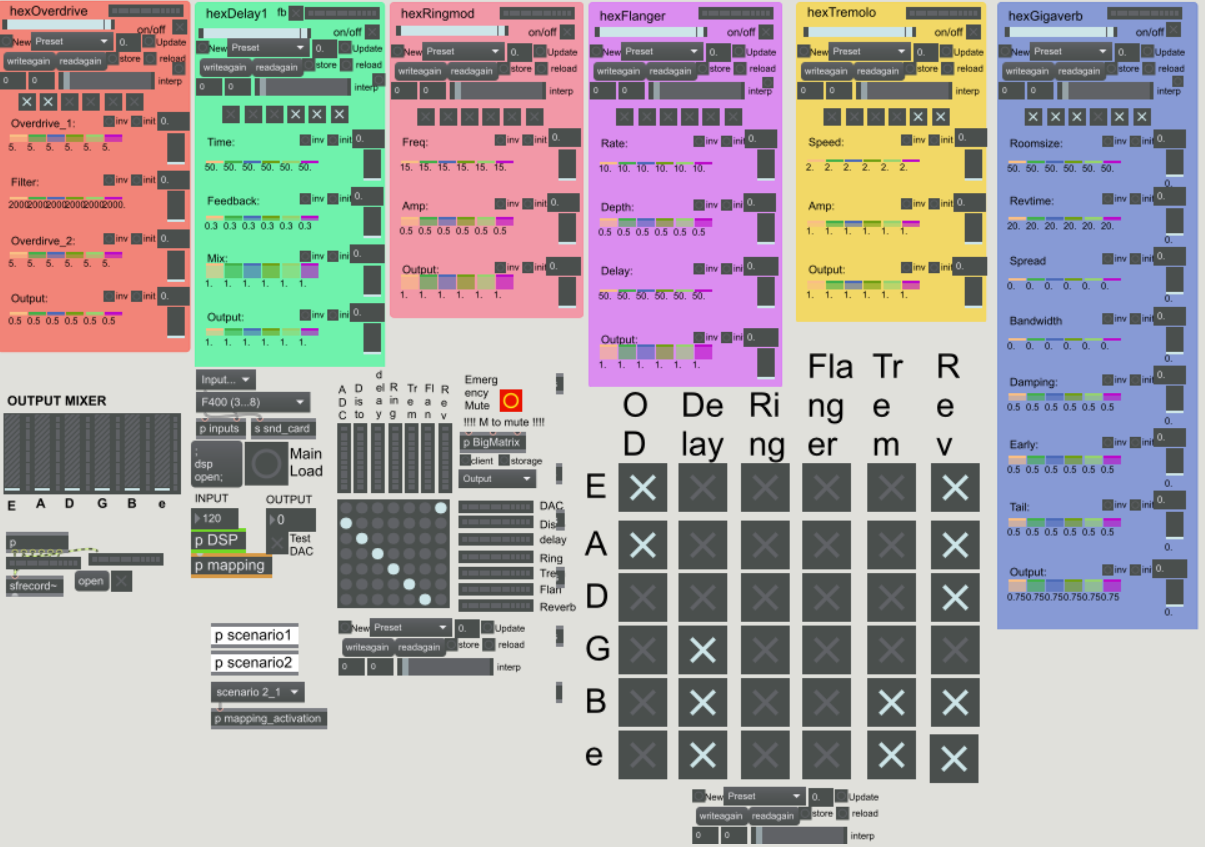
\includegraphics[width=\columnwidth]{figures/191025-Patch-experience.png}
    \caption{Hexaphonic Multi-Effects used for the experiments.}
    \label{fig:hex-multieffect}
\end{figure}

Multiple audio and video files were recorded during the experiment. 
On the audio side, the hexaphonic audio signals were recorded before (``dry" or ``clean") and after \linebreak(``wet"\footnote{The ``wet" term is often present in effects like reverb for example where levels of modified signals and non modified signals can be modified. In this context, this term refers to the level of the modified signal.}) the chosen audio effects. As the result, the clean hexaphonic signals enable to easily use any type of algorithm detection to ease the annotation part and the wet hexaphonic signals give a detailed look at the produced sound. A monophonic reduction of the hexaphonic wet signals was also recorded in order to have a low quality format easier to work with (only the two first channels of hexaphonic audio files can be heard when listen to through audio player software).
Moreover, the guitarist was asked to start (when ready) a mono mix recording of its improvisation. 
On the video side, a Nikon 5D mark IV camera was used to capture the guitarists while the were playing (during test, improvisation or interview parts). Video files were recorded with a resolution of 1920x1080 at 25 fps. The screen of the computer, on which the audio program ran, was also recorded in order to keep track of the user changes to the program GUI. The video conference software Zoom was used for that purpose so that recordings could be launched remotely without having the guitarist to do it.

All recorded signals were synced by sound. The guitarist was asked to pluck the lowest string with a palm-muting technique in order to record on each media a sharp event that can easily be detected and refered to.

\section{Dataset}\label{sec:dataset}
Once all those raw signals are recorded, several steps are necessary in order to obtain a useable dataset. 

The first step was to extract from recorded audio and video files, the media corresponding to each specific sub-scenario recordings. Syncing points (made by plucking the palm-muted lowest string), as well as timings of sub-scenarios parts (test, recordings or interviews) were annotated by hand in order to automatically trim and export files corresponding to each sub-scenario. The trim and export steps were done using \texttt{ffmpeg}\footnote{\url{https://www.ffmpeg.org/} (08/02/2022).} and \texttt{sox}\footnote{\url{http://sox.sourceforge.net/} (08/02/2022).} softwares, respectively for dealing with video and audio files. Each part of each sub-scenario is then made out of 5 files: 
\begin{itemize}
\item 2 video files: one from the camera, one from the computer screen;
\item 3 audio files: clean and wet hexaphonic signals as well as monophonic mix down of wet hexaphonic signals.
\end{itemize}  

The second step was to annotate each sub-scenario. Different types of annotations were used for different types of collected data: 
\begin{itemize}
\item Global information, such as scenario and sub-scenario number, instrument tuning (and its evolution if necessary), duration of the specific part, used audio effects and presets, were collected;

\item Played notes have been retrieved by using a semi-automatic method similar to the one used in \cite{sci:Xi2018}. Six automatic pitch extractions were performed in parallel, on the hexaphonic clean signals. As tuning (i.e., pitches of the strings when no notes are fretted) of the guitar was known, fret number was inferred from pitch extraction result and string number.  \texttt{Aubio} library's\footnote{\url{https://aubio.org/} (08/02/2022).} implementation of \texttt{yin-fft} algorithm \cite{sci:Brossier_yinFFT} has been used to perform this task\footnote{It has to be noticed that different pitch detection algorithms were tested inside of Sonic Visualizer software and that the \texttt{yin-fft} algorithm appeared to give the best results. }. The data generated by the algorithm have then been manually verified in order to consolidate notes and frets information; 

\item The activation periods of each individual effects from scenario 2 have been automatically extracted from computer screen videos. A computer vision algorithm has been built to track the changes in the indivual bypasses of hexaphonic effects of the graphical user interface (thoses changes have then been computed as time segments). Moreover, in order to be able to easily visualize those changes with the improvisation, the global bypass matrix from the computer screen videos has been cropped and overlayed on top of the camera video; %(see Figure \ref{fig:overlay})

\item Common guitar playing techniques, such as bend, harmonics, hammer-on, pull-off, etc. (see, e.g \cite{sci:Su2014a}, for details on such techniques), have been manually annotated. Extended playing techniques like use of a bow,objects or preparations as well as more advanced techniques like \textit{scordatura}\footnote{The \textit{scordatura} is the action of strongly detuning the strings in order to be able to play with
the timbres generated in part by the softness of the relaxed strings.} are also including in the annotations. Definitions and explanations of those kind of extended or advanced techniques can be found in \cite{Josel2014},  \cite{organo:schndeider2015_microtones} and \cite{organo:Landman2012} or \cite{organo:ElgartYates1990}. To the best of our knowledge, these kind of techniques are most often not present in litterature's datasets.
\end{itemize}

%\begin{figure}
%    \centering
%    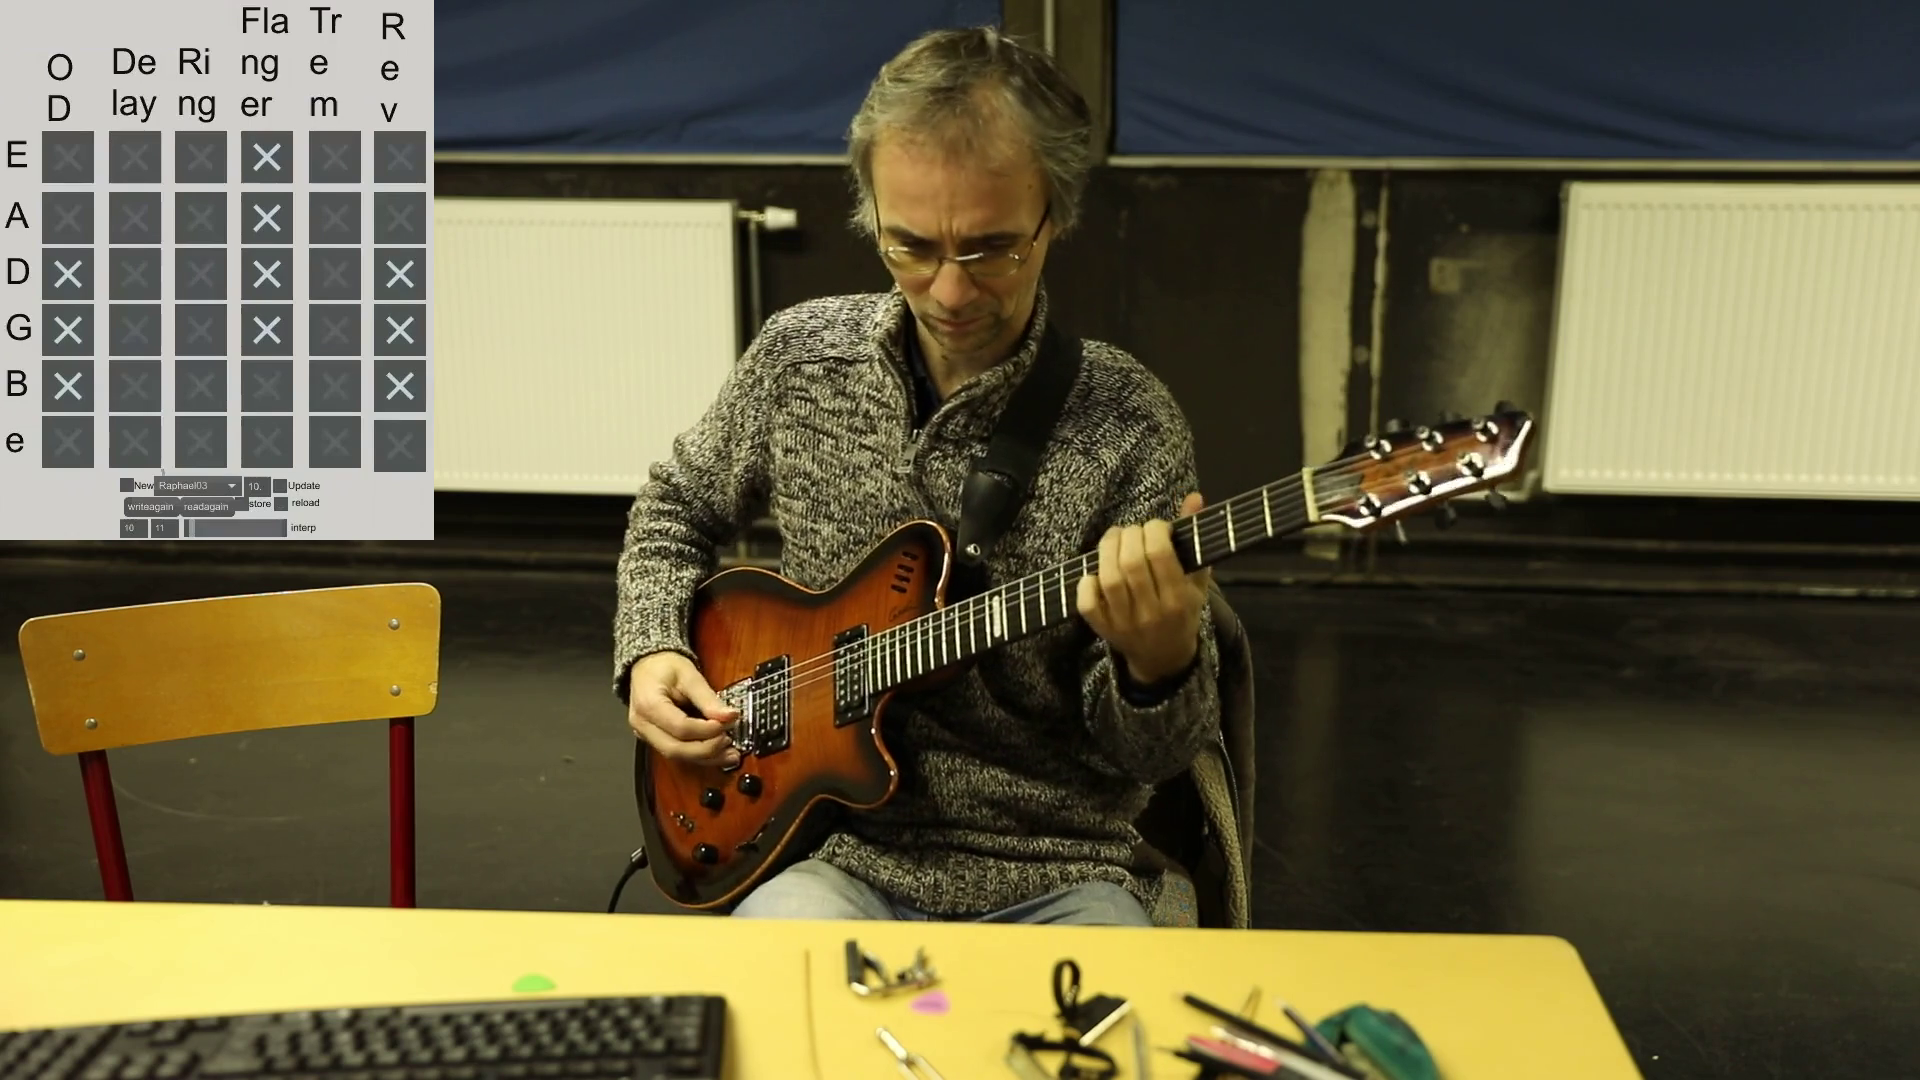
\includegraphics[width=\columnwidth]{figures/Raphael-2_5-rec-impro_01-screenshot-00_05_30_800}
%    \caption{Bypasses matrix being overlayed on top of guitarist's performance.}
%    \label{fig:overlay}
%\end{figure}

All the data detailed above are stored in various file formats (\texttt{json}, \texttt{txt} or \texttt{csv}) in order to be compatible with different visualisation software like Sonic Visualizer\footnote{\url{https://www.sonicvisualiser.org/} (08/02/2022).} or Advene\footnote{\url{https://www.advene.org/} (08/02/2022).}. An exemple of the collected data integrated in Advene software can be seen on Figure \ref{fig:Ivann-2_4-advene}. %It has to be noticed that at the time of the writing the complete data collection is not complete.

To complete the objective collected data, interviews made after each improvisations have been transcribed.  The me\-thod used for the transcription is the one of the verbatim. The use of the verbatim here is made so that researchers from other fields willing to analyze those texts can access the data in minimally modified form. Only some common french oral language words or expressions have been rewritten with more readable terms. The analysis that we are making in next section is specifically based on those transcriptions. 


% ?
%The global dataset provides 10 hours of guitarists improvisations (audio -hexaphonic and monophonic format- and video recordings) using an hexaphonic multieffect as well as 4 hours and 30 minutes of interview have been transcribed.

%In order to facilitate further analysis of the improvisation, visual feedback for audio effects activation segments were added to the improvisations video file. An example of such an integration can be seen on figure \ref{fig:Ivann-2_4-timeline}.

\begin{figure}
    \centering
    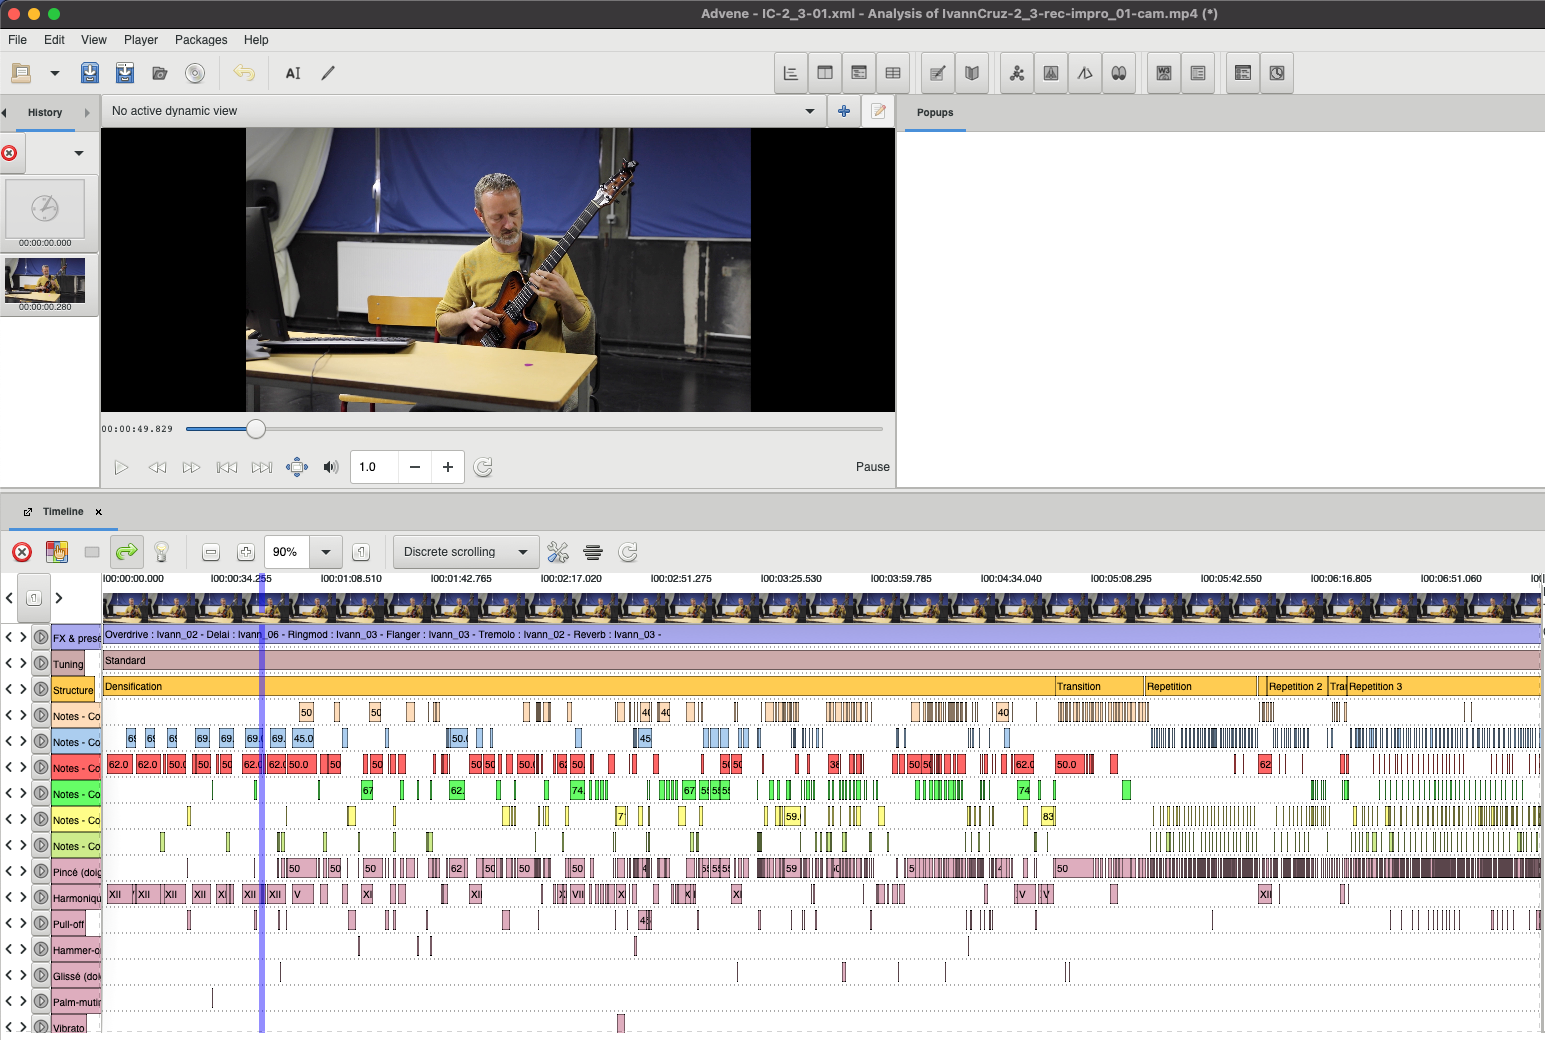
\includegraphics[width=\columnwidth]{figures/IvannCruz_2_3_1_Advene.png}
    \caption{GIHME annotations integration example in Advene software.}
    \label{fig:Ivann-2_4-advene}
\end{figure}
%total duration of improvisation, total duration of interviews, features (onset, offset, string, fret, tuning), etc.


%\begin{itemize}
%    \item synchronisation points annotation and use of script to automatically sync all the medias for a given sub-scenario. Screen video have been resampled so that it matches the camera resolution and fps rate.
    
%    \item string/fret : played fret number has been automatically inferred from hexaphonic signals using a script performing automatic pitch recognition. The result of this script is then human verified.
    
 %   \item computer vision techniques have been used and screen videos in order to capture and annotate the use of strings with effects vs strings without effect in the first scenario and activated bypasses in the second scenario.
%\end{itemize}


\section{Interviews analysis}
\label{sec:analysis}

This analysis of the words of the guitarists is a first step towards understanding and characterizing their practices have been altered by the use of the hexaphonic multieffect.  
%Let us remind, that the number of guitarists involved in those experiments is pretty small (five). 
The different points presented below give good hints about the impact of hexaphonic multieffect on practices of guitarists, but, for now, it cannot be easily generalizable as the number of guitarists who participate in that experiment is pretty small.

%\subsection{Biases}
%The experiment introduces several biases which have to be taken into account.
%
%The first one is the duration of the experiment. Three days per guitarist is a limited amount of time that enables the guitarists to have a good first idea of the artistic potentials of the system but not to develop a specific practice with new modes of playing for example. Guitarist number 5 clearly stated that more time would have been the solution to find more ideas for each scenario. 
%
%\begin{quote}
%    "I think I could get something out of it, but I would need more time [...]. I would need to play it everyday in order to find stuff that I like. (Guitarist 5, extract from post-improvisation interview, scénario2\_5, pers. comm.)
%\end{quote}
%%Alexandre Antoine
%
%%\begin{quote}
%%    "Je pense que c'est beaucoup de boulot [...]. Je ne sais pas si au final [...] ça peut me servir pour moi ce que je fais, pour l'utilisation que j'ai de la guitare. [...] Je pense que je pourrais arriver à quelque-chose, mais il faudrait beaucoup plus de temps. [...] Faudrait que j'en fasse tous les jours pour trouver un truc qui me plait.(Alexandre Antoine, extrait interview post-improvisation, scénario2\_5)"
%%\end{quote}
%
%The number of guitarists is also quite limited due to economic reasons. The analysis coming out from this dataset therefore cannot be easily generalized.  
%
%Practice of each guitarist was partially known by the researcher and several parts of the interviews are questions related to understanding whether or not the different techniques they used were part of their practices or were induced by the system.


%
%    \begin{quote}
%        "Là comme t’alternes tu sais pas trop sur quel pied danser, donc euh […], ouais faut vraiment réinventer une façon de jouer. (extrait interview post-improvisation, scénario1\_3, Sébastien Beaumont)"
%    \end{quote}
    
%Necessity of having a practice developed enough to extract the most of hexaphony and hexaphonic processing.
%Strong tool to enhance performance of guitarists with timbral approach to guitar 

%Several of them used various techniques to simplify the complexity of the different scenarios : not a lot of techniques (tapping + tremolo) for SB, detuning of strings to obtain 2 or 3 harmonic distinct poles (RG), focused on 2 or 3 strings (PL)

\subsection{Constraints and limitations}
Before talking about the impact of the hexaphonic multieffect itself, one common element to all guitarists is that, at some point, they felt constrained. The limitations they endured were most of the time either due to the configurations of scenarios or to the technical elements used for the experiment.

It has to be noticed that the scenarios and sub-scenarios configurations do act as constraints already, as they put all the guitarists in unusual situations, but most of the time the guitarists have managed to work with them and felt stimulated by them. The constraints listed below are the ones where guitarists had a hard-time integrating those configuration in their improvisations.

Regarding to the hexaphonic, multieffect several constraints were mentioned : the balance between the volume of dry strings and strings on which effects were applied in scenario 1 was, for example, mentioned by guitarists 1 and 3 as being problematic (the issue was resolved by adding the output mixer mentioned in Section \ref{sec:hex_multifx}). Some effects configurations were felt uneasy : guitarist 1 had trouble playing with different delay times when those were not rhythmically related and guitarist 5 felt that applying distortion only on specific strings was not a natural fit for him. 

On the scenario level, all the manipulations needed to access the different individual bypasses in scenarios 2\_3, 2\_4 and 2\_5 (due to the use a foot controller FCB1010 as mentioned above) was mentioned by guitarists 1, 4 and 5 as being not intuitive and adding a strong inertia to the whole process.
Guitarist 2 felt a strong constraint with effects distribution in scenario1\_3 and 1\_4:
%    \begin{quote}
%        "je me retrouve un peu démuni en fait devant une configuration comme celle-là. Donc euh, j’ai mes réflexes de, de, de guitariste […] qui essaient d’aller chercher quelque-chose mais qui n’est plus là. Donc euh, oui ça essaie, ça pointe son nez, mais ça marche pas [silence]." (extrait interview post-improvisation, scénario1\_3-02, Sébastien Beaumont)
%    \end{quote}
    \begin{quote}
        I was a bit helpless in fact with a setup like this one. [...] I have my guitarist's reflexes that try to find something but which is not there anymore. So, yeah it tries [...], but it doesn't work. (Guitarist 2, extract of post improvisation interview, scenario1\_3-02, pers. comm.).
    \end{quote}
    %%%% Sébastien Beaumont

One last type of constraint is due to acoustic and electric behavior of the piezoelectric hexaphonic pickup. Indeed cross-talk\footnote{A small amount of the sound of a vibrating string is picked up by adjacent pickups.} and transfer of a played string's vibrations to other pickups through the bridge create resonances on non-played strings. These two phenomena are particularly significant in scenario 1, where notes played on strings without effects would trigger low volume modified sounds on strings with effects. This is especially true when the distortion is used on the string with effects as it increases the volume of the strings.
However, these constraints were used by guitarist 2, 3 and 4 as a mode of playing in itself. 

%Alongside with this specific adaptation, it has to be noticed, that most constraints felt by guitarists regarding the scenarios' specificity were integrated and resolved along the run through the sub-scenarios. These resolutions appeared most of the times after guitarist's acceptance of the system specificities. As guitarist one stated : 
%    \begin{quote}
%        "I was a bit helpless in fact with a setup like this one. [...] I have my guitarist's reflexes that try to find something but which is not there anymore. So, yeah it tries [...], but it doesn't work. (Sébastien Beaumont, extract of post improvisation interview, scenario1\_3-02, pers. comm.)."
%    \end{quote}

%Foot controller


\subsection{Appropriation of the system}

In spite of the constraints brought by the scenarios and by the technical system, the guitarists have, for the great majority, succeeded in appropriating and integrating the complexity of the system. They have, for the most part, put in place various strategies to reduce this complexity.

%\subsubsection{Strategies to reduce complexity}
Guitarist 3, for example, played several improvisations using only a limited amount of prepared strings\footnote{Instrument's preparation is the process by which object are added or fixed on the strings in order to modify its original timbre.} (scenario 1\_2) or a limited way to attack the strings (scenarios 2\_1, 2\_2, 2\_3). In scenario 1\_2, guitarist 4 used preparation (a small bar of metal inserted in between the strings close to the bridge)\footnote{See video recording at \url{https://vimeo.com/639069813} (08/02/2022).} on the three dry strings in order to bring their timbre closer to the ones of the strings with effects. The same guitarist used \textit{scordatura} right from the beginning (scenario 1\_1) to limit the harmonic range of the guitar\footnote{See video recordings at \url{https://vimeo.com/639069333} (08/02/2022).}:
    \begin{quote}
     It appeared to me as a way, in this chaos of the low strings [strings with effects, editor's note], to try to find an organization clearer for me. (Guitarist 4, extract of post improvisation interview, scenario1\_1, pers. comm.).
    \end{quote}
In this improvisation, the standard tuning of the guitar, E-A-D-G-B-e, evolved to E-A-D-A-A-e (the D string was left unused during all the improvisation). 

During scenario's test step, guitarist 5 played pieces of his repertoire while applying effects in a random manner. Both of these actions (know pieces playing and randomness) helped him to dig directly into hexaphonic effects timbre without overthinking too much. From there he narrowed down to specific choice of effects and presets as well as specific directions for his improvisations (most of the time inspired by the pieces he just played). 

\subsection{Guitarist practice}
The playing of an electric guitar is necessarily modified by the addition of an hexaphonic microphone and of an string-individualized sound processing system. The gestures made by the guitarists no longer have the same scope, the same impact, which leads him to reexamine his relationship with his instrument and therefore his practice.
However hexaphonic multieffect practice was not considered by the guitarists as something radically new.  As guitarist 2 stated: ``it's another instrument, but at the same time, it's a familiar one"\footnote{Guitarist 2, extract of post improvisation interview,  scenario 2\_5, pers.comm}. 

Guitarist 4 notes the sensitivity of the hexaphonic pickup ``regarding the reactivity [...], it's very sensistive [he plucks the strings very slighlty with his nails, editor's note]"\footnote{Guitarist 4, extract of post improvisation interview,  scenario 1\_5, pers.comm}. The hexaphonic pickup on this guitar are piezoelectric ones. Those type of pickups sense a broader frequency spectrum \cite{sci:Lemme_SoundSecret_electricGuitar} than most of the regular electromagnetic pickups found on electric guitars. 
But what this very technical remark highlights is that this kind of pickup is very good at sensing all subtleties of guitarist's playing. This element is very important in terms of respect of practice and acceptance of hexaphony by guitarists. 


Guitarist 1 develops the same idea :

%\begin{quote}
%	``[. . . ] it's another instrument, but at the same time, it's a familiar one". (Guitarist 2, extract of post improvisation interview,  scénario 2\_5, pers.comm).
%  ``[. . . ] c’est un autre instrument, mais en m me temps, qui m’est familier [. . . ]"  . Interview post-sc nario 2_5, S bastien Beaumont, communication personnelle.
%\end{quote}

\begin{quote}
[...] because there's also the habit of linking instrumental gesture with foot gestures on the pedals. So there you have it, it seems to me to fit more into the same logic, but at a higher level we'll say. (Additional interview, Guitarist 1, pers.comm).
%	``[...] parce que y’a aussi l’habitude de, de lier le geste instrumental avec des jeux de pieds sur des pédales. Donc voilà, ça me paraît plus rentrer dans la même logique, mais à un niveau supérieur on va dire." Additional interview, Ivann Cruz, pers.comm.
%	``[...] parce que y’a aussi l’habitude de, de lier le geste instrumental avec des jeux de pieds sur des pédales. Donc voilà, ça me paraît plus rentrer dans la même logique, mais à un niveau supérieur on va dire." Complément d'interview, Ivann Cruz, pers.comm.
\end{quote}

With this quote, guitarist 1 emphasizes that working with the foot controller in scenario 2 is pretty close to its practice of monophonic guitar effect pedals but it adds more relief or details to it. This idea of being part of a known and familiar practice which goes further and needs to adpat is developped by guitarist 2 : 

    \begin{quote}
     It doesn't question the pratice. The practice, it stays, it exists. However, it reconsiders it, in the sense where, as new things happen, you have to adapt. [...] It's a system who forces you to look deeply at the instrument for ways to adapt, even if it is a material that I know. I mean, all this effects, I've already used them in my life. They are part of the guitarist's landscape. And despite all that, the fact to use them in hexaphony, you rethink the effects differently too. You rethink, you adapt your playing, an interaction takes place. (Guitarist 2, extract of post improvisation interview, scenario2\_5, pers. comm.).
    \end{quote}

The same guitarist sums up this idea in a pretty concise and concrete way when he mentions ``with this system, you have to redraw the geographical relationship with your instrument"\footnote{Additional interview, Guitarist 1, pers. comm.}. This ``geographical relationship" is close to the notion of ``mapping" often used in NIME (New Interface for Musical Expression) context. Using an hexaphonic multieffect pushes the guitarist to modify the relationship, one could say the ``inner mapping", he has built between his gesture and the produced sound. 

From these few excerpts, it appears that this hexaphonic setup can easily integrate into practices of guitarists as it uses the same elements as their regular pratices, but they also need to adapt this practice in terms of relationship between the gesture and the produced sound.

%\begin{quote}
%``tu dois redessiner le rapport géographique à l’instrument avec ton système [...]". Complément d’information, Sébastien Beaumont, communication personnelle.
%\end{quote}



\subsection{Hexaphonic specificities}

Regarding the produced sounds, several comments develop the idea of this setup having a rich palette of sounds. Guitarists 1 and 4 both make the parallel with the organ. This metaphor derives direclty from the use of the foot controller in the second scenario but also from the vast amount of sounds accessible through this controller  and through the playing.  Let's remember that scenario 2\_5 gives access to individual bypass control of individual effects as well as to presets of the whole bypass matrix. These options gives the musicians the ability to change completely configurations or just to make tiny adjustments, these abilities being modulated by guitarist's playing which itself acts as a ``selection gesture" \cite{sci:Cadoz94} inside of the defined timbre palette.
Guitarist 2 develops this idea by comparing the sound possibilities to the ones given by digital audio workstation (DAW) : 

\begin{quote}
Precisely, it helps going into fields that could be covered by the digital world and all that.  I find that we come close to things like that, while respecting the instrumental practice.  [...] I'm not saying that it's like MIDI [...], it's a kind of in-between.  (Guitarist 2, extract of post improvisation interview, scenario2\_5, pers. comm.)
%Justement,  a permet d’aller vers des champs qui pourraient  tre
%offerts par le num rique et tout  a. Je trouve qu’on s’approche de
%choses comme  a, tout en respectant la pratique instrumentale.
\end{quote}

``Respect of instrumental practice" referred by guitarist 2 echoes remarks from the previous part, but also comes in opposition to MIDI control of instruments. With the hexaphonic system, the guitarist uses the professionnal practice he spent years to develop to access all these sound possibilities.

The specificities of the practices used during this experiments are also the center of the last hexaphonic specificity developed here. Indeed, it appears that practices that already made use of techniques to develop polyphonic or multitimbral approaches of the guitar were enhanced by this system. 
Guitarist 3 who extensively used preparations during its improvisation points out at several moments the gain of clarity due to the hexaphony : 

\begin{quote}
[...] one can add a tremolo or a delay on just one string, it's really nice. Or a reverb on one string, it brings a bit of depth and it won't impact everything. On a classic annalog effect, it necessarily take huge proportion. Here, one can add a huge reverb, but just on one string, it's very convenient yeah. (Guitarist 4, extract of post improvisation interview, scenario2\_4-01, pers. comm.).
\end{quote}

Despite being obvious when said out loud, this remark brings to the fore the idea that monophonic effect pedals are not that well-suited for prepared guitar practice. Indeed, added preparations can be string specific (as well as applied to multiple strings) whereas monophonic effects do apply to all the strings at the same time.
In such a context, string specific effect system (aka hexaphonic multieffect) brings a natural continuity to preparations.
Guitarist 4 whose practice fals into classical, contemporary and flamenca styles tends to formulate the same kind of idea: 

\begin{quote}
With a classical guitar, we work with the aim of being able to have an action as independent as possible from each finger and therefore potentially also differentiated regarding the strings. (Guitarist 4, complementary interview, pers. comm.).
\end{quote}
%sur la guitare classique on travaille dans le but de pouvoir
%avoir une action la plus ind pendante possible de chaque doigt, et
%donc potentiellement diff renci e  galement par rapport aux cordes.
%[...] apr s il faut savoir malgr  tout que beaucoup de guitaristes
%cherchent encore l’homog n it  la plus parfaite qui puisse  tre trouv e
%sur l’instrument. [...] il y a aussi tout un tas de guitaristes qui
%jouent de la musique contemporaine et qui donc appr cient cette
%recherche de diversit  de timbres, d’ nergie, de polyphonie.  . Compl ment
%interview, Rapha l Godeau, communication personnelle.

This quote comes as a justification of the idea brings by guitarist 4 that the hexaphonic multieffect setup could be of interest of classical guitarists who would want to move on electric guitar. As he mentions, the independence of the finger from each other seems to find a continuity in a string specific audio effects system. This point (that wasn't expected in the first place) and the example of the prepared guitar practice seems to highlight that this kind of system is a good fit for practices that seeks for independance in terms of gestures, of strings or of preparations.

%Indeed as not all preparations fits a specific monophonic effect, extra manipulations would be needed in order to apply it to specific preparations. With the possibility to configure independently each string, guitarists who use preparations can prepare them and their associated effects in advance, without the obligation to think up their removal or installation.
%
%Guitarist 4 tends to approach its instrument specifically in timbre terms by the use of different types of attacks or by the use of scordatura. The latter, to him, finds a perfect continuity in the use of string-independent effects as it can emphasize the different timbres obtained by the reduction of the string tension. 

%Ça remet pas en cause la pratique. Ta pratique, elle reste, elle existe. Par contre, ça la remet en question dans le sens où, comme il se passe d’autres choses, il faut que tu t’adaptes

%c’est un dispositif qui euh, qui te force quand même à chercher sur l’instrument des moyens d’adaptation, alors que c’est un matériau finalement que je connais. Enfin, tous ces effets-là, je les avais déjà utilisés dans ma vie. Ils font partis du paysage euh, du guitariste. Et malgré tout, le fait de les utiliser en, en hexaphonie comme ça ben, [court silence] tu repenses aussi les effets différemment, tu repenses, t’adaptes ton jeu, enfin y’a une interaction qui se passe.

\section{Future work}\label{sec:future_work}

While bringing some important notions, this first analysis and this dataset could definitely be improved. Recordings coming from more guitarists with more different styles of music would help broaden the results. The different styles seem pretty important as other music styles come with specific modes of playing, which were not represented in this dataset. These different modes of playing could adapt differentely to hexaphonic effects.
We showed a data visualization test in Advene software, but this software, while being able to show all the data (except audio signals) at once, is not optimum to run a study with such a number of different types of data.  Being able to switch between audio signals (clean or wet hexaphonic, monophonic or sound from video) while looking at the same video or to summarize relevant data for specific parts of an improvisation are some of the features which would be really useful for this kind of study.
Lastly, the first insights gained by the anaysis of the interviews could be broadened by the addition of the objective data and their analysis. The use of a fretboard patterns analysis tool such as the model developed in \cite{musico:deSouza2018_fretboard} could help in finding a common ground to the different practices analysis. Further, in order to really understand the impact of the hexaphonic setup on the practice of one specific guitarist, an analysis of its regular practice (i.e. without hexpahonic setup) should be done so as to enable a "before/after" comparison.

\section{Conclusion}\label{sec:conclusion}
This paper presents a novel dataset including improvisations of 5 different guitarists using hexaphonic guitar and multieffect. Such a system enables them to apply string-independent effects. This dataset gathers 10 hours of improvisations and transcription of 4.5 hours of interviews. 
Each sub-scenario's improvisation is annotated with pitch, string/fret, playing techniques (including extended techniques), effects configuration and effects activation timings. As these annotations represent a large amount of data, the first analysis given in this paper is based on the different interviews. According to the guitarists, this system, while new, appears to be familiar: effects are a well-known paradigm for electric guitarists and there's no need to learn new gestures; the guitarists' practices can be used as is. What requires a new approach from the guitarists, though, is the impact the instrumental gestures have on the generated sound, what one could call ``inner mapping".  Indeed by being string-specific, hexaphonic effects add another level to the impact the gestures can have.
As a wrap-up, guitarists make several remarks that tends to emphasize that this system is particularly relevant with practices that already use extensively the independance of fingers and strings, such as prepared or classical guitare practices.



\begin{acknowledgments}
I'd like to thank Livio Ratti, student at the University of Lille (France) for his precious help during the recording sessions and the derush step. 

This work was partially funded by Region Wallonne and EU, in the framework of ERDF project DigiSTORM.
\end{acknowledgments} 

%%%%%%%%%%%%%%%%%%%%%%%%%%%%%%%%%%%%%%%%%%%%%%%%%%%%%%%%%%%%%%%%%%%%%%%%%%%%%
%bibliography here
\bibliography{GIHME-SMC2022-bibliography}

\end{document}

%%%%%%%%%%%%%%%%%%%% FROM TEMPLATE
%\section{Page size and format}
%\label{sec:page_size}
%The SMC 2022 proceedings will be formatted as portrait \underline{A4-size papers (21.0~cm x 29.7~cm)}. All material on each page should fit within a rectangle of 17.2~cm x 25.2~cm, centered on the page, beginning 2.0~cm from the top of the page and ending with 2.5~cm from the bottom. The left and right margins should be 1.9~cm. The text should be in two 8.2~cm columns with a 0.8~cm gutter. All text must be in a two-column format, and justified.
%
%Papers should be between 4 and 8 pages, written in English, and not previously published. Papers must be submitted as PDF documents generated using the provided \LaTeX{} or Word templates.
%
%
%\section{Typeset Text}\label{sec:typeset_text}
%
%\subsection{Normal or Body Text}
%\label{subsec:body}
%Please use a 10~pt (point) Times font. Use sans-serif or non-proportional fonts only for special purposes, such as distinguishing source code.
%
%The first paragraph in each section should not be indented, 
%but all other paragraphs should be.
%
%\subsection{Title and Authors}
%The title is 16~pt Times, bold, caps, upper case, centered. Authors' names are centered. The lead author's name is to be listed first (left-most), and the co-authors' names after. If the addresses for all authors are the same, include the address only once, centered. If the authors have different addresses, put the addresses, evenly spaced, under each authors' name.
%
%\subsection{First Page Copyright Notice}
%Please leave the copyright notice exactly as it appears in the lower left-hand corner of the first page. Make sure to update the first author’s name in the copyright notice, accordingly. It is set in 8~pt Times.
%
%\subsection{Page Numbering, Headers and Footers}
%Do not include headers, footers or page numbers in your submission. These will be added electronically at a later stage, when the publications are assembled.
%
%\section{Headings}
%First level headings are in Times 12~pt bold, centered with 1 line of space above the section head, and 1/2 space below it.
%For a section header immediately followed by a subsection header, the space should be merged.
%
%\subsection{Second Level Headings}
%Second level headings are in Times 10~pt bold, flush left, with 1 line of space above the section head, and 1/2 space below it. The first letter of each significant word is capitalized.
%
%\subsubsection{Third Level Headings}
%Third level headings are in Times 10~pt italic, flush left, with 1/2 line of space above the section head, and 1/2 space below it. The first letter of significant words is capitalized.
%
%Using more than three levels of headings is strongly discouraged.
%
%
%
%
%
%\section{Floats and equations}
%
%\subsection{Equations}
%Equations should be placed on separated lines and numbered. The number should be on the right side, in parentheses.
%\begin{equation}
%r=\sqrt[13]{3}
%\label{eq:BP}
%\end{equation}
%Always refer to equations like this: ``Equation (\ref{eq:BP}) is of particular interest because...''
%
%\subsection{Figures, Tables and Captions}
%\begin{table}[t]
% \begin{center}
% \begin{tabular}{|l|l|}
%  \hline
%  String value & Numeric value \\
%  \hline
%  Moin! SMC & 2022 \\
%  \hline
% \end{tabular}
%\end{center}
% \caption{Table captions should be placed below the table,  like this.}
% \label{tab:example}
%\end{table}
%
%All artwork must be centered, neat, clean and legible. Figures should be centered, neat, clean
%and completely legible. All lines should be thick and dark enough for purposes of reproduction. Artwork should not be hand-drawn. The proceedings will be distributed in electronic form only, therefore color figures are allowed. However, you may want to check that your figures are understandable even if they are printed in black-and-white.
%
%
%Numbers and captions of figures and tables always appear below the figure/table.
%Leave 1 line space between the figure or table and the caption.
%Figure and tables are numbered consecutively. 
%Captions should be Times 10pt. Place tables/figures in the text as close to the reference as possible, 
%and preferably at the top of the page.
%
%Always refer to tables and figures in the main text, for example: ``see Fig. \ref{fig:example} and \tabref{tab:example}''.
%Figures and tables may extend across both columns to a maximum width of 17.2cm.
%
%Vectorial figures are preferred, e.g., eps. When using \texttt{Matlab}, export using either (encapsulated) Postscript or PDF format. In order to optimize readability, the font size of text within a figure should be no smaller than
%that of footnotes (8~pt font-size). If you use bitmap figures, make sure that the resolution is high enough for print quality. 
%
%\begin{figure}[t]
%\centering
%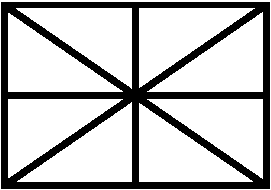
\includegraphics[width=0.6\columnwidth]{figure}
%\caption{Figure captions should be placed below the figure, 
%exactly like this.\label{fig:example}}
%\end{figure}
%
%
%\subsection{Footnotes}
%You can indicate footnotes with a number in the text \footnote{This is a footnote example.},
%but try to work the content into the main text.Use 8~pt font-size for footnotes.  Place the footnotes at the bottom of the page 
%on which they appear. Precede the footnote with a 0.5~pt horizontal rule.
%
%\section{Citations}
%All bibliographical references should be listed at the end, inside a section named ``REFERENCES''. References must be numbered in order of appearance. You should avoid listing references that do not appear in the text.
%
%Reference numbers in the text should appear within square brackets, such as in~\cite{Someone:00} or~\cite{Someone:00,Someone:04,Someone:09}. The reference format is the standard IEEE one. We highly recommend you use BibTeX 
%to generate the reference list.
%
%\section{Conclusions}
%Please, submit full-length papers. Submission is fully electronic and automated through the Conference Web Submission System. \underline{Do not} send papers directly by e-mail.
